% IEEE Paper Template for US-LETTER Page Size (V1)
% Sample Conference Paper using IEEE LaTeX style file for US-LETTER pagesize.
% Copyright (C) 2006-2008 Causal Productions Pty Ltd.
% Permission is granted to distribute and revise this file provided that
% this header remains intact.
%
% REVISION HISTORY
% 20080211 changed some space characters in the title-author block
%
\documentclass[10pt,conference,letterpaper]{IEEEtran}
\usepackage{times,amsmath,epsfig}

\usepackage{graphicx}
\usepackage{hyperref}
\usepackage{booktabs}
%
\title{Movie recommendation: Collaborative Filtering}
%
\author{
{Vishal Anand (UNI: va2361)}
\vspace{1.6mm}\\
\fontsize{10}{10}\selectfont\itshape
Department of Computer Science, Columbia University\\
New York City, NY, USA\\
\fontsize{9}{9}\selectfont\ttfamily\upshape
vishal.anand@columbia.edu}
%
\begin{document}
\maketitle
%
\begin{abstract} 
As part of homework 1 of COMS-6998 : Advanced Machine Learning with Personalization, a movie recommendation engine is built which performs collaborative filtering. The rank matrices are factorized and completed by decomposing through low-rank factorization.
\end{abstract}

\section{Introduction}
We are working on the \href{http://files.grouplens.org/datasets/movielens/ml-20m.zip}{MovieLens 20M dataset} which contains 20000263 ratings across 27278 movies as generated by 138493 users between January 09, 1995 to March 31, 2015. All selected users have rated at least 20 movies. The file ratings.csv contains the ratings given to some movies on a 5-star scale with half-increments. On each line, the file has a rating with the following format (userId;movieId;rating;timestamp).

\begin{itemize}
\item The entire movie-ratings data-set and was split randomly with 50\% of each user in test/train sets respectively.
\item Five different splits of data were generated through this process
\end{itemize}

\section{RMSETest, RMSETrain, MRR Data Produced: Pre-Analysis}
The other Split datas are located in the appendix
\subsection{Split-1}
\begin{table}[h!] \begin{tabular}{rrrrrr}
\toprule
 Rank &  Lambda &  Iter &  RMSE\_train &  RMSE\_test &       MRR \\
\midrule
   10 &   0.001 &     1 &    1.038286 &   0.953560 &  0.144645 \\
   10 &   0.001 &     2 &    0.920051 &   0.907733 &  0.144786 \\
   10 &   0.001 &     3 &    0.891892 &   0.891609 &  0.144810 \\
   10 &   0.001 &     4 &    0.879021 &   0.883577 &  0.144815 \\
   10 &   0.001 &     5 &    0.871695 &   0.878953 &  0.144821 \\
   10 &   0.001 &     6 &    0.867026 &   0.876059 &  0.144823 \\
   10 &   0.001 &     7 &    0.863824 &   0.874144 &  0.144818 \\
   10 &   0.001 &     8 &    0.861506 &   0.872826 &  0.144818 \\
   10 &   0.001 &     9 &    0.859752 &   0.871889 &  0.144813 \\
   10 &   0.001 &    10 &    0.858373 &   0.871202 &  0.144809 \\
   10 &   0.001 &    11 &    0.857244 &   0.870679 &  0.144803 \\
   10 &   0.001 &    12 &    0.856283 &   0.870260 &  0.144797 \\
   10 &   0.001 &    13 &    0.855425 &   0.869898 &  0.144789 \\
   10 &   0.001 &    14 &    0.854620 &   0.869553 &  0.144789 \\
   10 &   0.001 &    15 &    0.853821 &   0.869186 &  0.144783 \\
   10 &   0.001 &    16 &    0.852982 &   0.868757 &  0.144765 \\
   10 &   0.001 &    17 &    0.852056 &   0.868226 &  0.144768 \\
   10 &   0.001 &    18 &    0.850996 &   0.867553 &  0.144765 \\
   10 &   0.001 &    19 &    0.849760 &   0.866707 &  0.144755 \\
   10 &   0.001 &    20 &    0.848324 &   0.865678 &  0.144751 \\
\bottomrule
\end{tabular}

\caption{split1: Rank=10, $\lambda$=0.001}
 \end{table}
\begin{table}[h!] \begin{tabular}{rrrrrr}
\toprule
 Rank &  Lambda &  Iter &  RMSE\_train &  RMSE\_test &       MRR \\
\midrule
   10 &    0.02 &     1 &    1.039179 &   0.950775 &  0.144744 \\
   10 &    0.02 &     2 &    0.919648 &   0.906044 &  0.144821 \\
   10 &    0.02 &     3 &    0.891683 &   0.890161 &  0.144827 \\
   10 &    0.02 &     4 &    0.878897 &   0.882247 &  0.144842 \\
   10 &    0.02 &     5 &    0.871627 &   0.877696 &  0.144857 \\
   10 &    0.02 &     6 &    0.867002 &   0.874848 &  0.144851 \\
   10 &    0.02 &     7 &    0.863839 &   0.872963 &  0.144856 \\
   10 &    0.02 &     8 &    0.861558 &   0.871662 &  0.144858 \\
   10 &    0.02 &     9 &    0.859842 &   0.870732 &  0.144851 \\
   10 &    0.02 &    10 &    0.858503 &   0.870045 &  0.144842 \\
   10 &    0.02 &    11 &    0.857419 &   0.869519 &  0.144840 \\
   10 &    0.02 &    12 &    0.856511 &   0.869096 &  0.144841 \\
   10 &    0.02 &    13 &    0.855717 &   0.868735 &  0.144840 \\
   10 &    0.02 &    14 &    0.854993 &   0.868401 &  0.144841 \\
   10 &    0.02 &    15 &    0.854298 &   0.868062 &  0.144843 \\
   10 &    0.02 &    16 &    0.853594 &   0.867686 &  0.144841 \\
   10 &    0.02 &    17 &    0.852843 &   0.867242 &  0.144840 \\
   10 &    0.02 &    18 &    0.852007 &   0.866695 &  0.144831 \\
   10 &    0.02 &    19 &    0.851046 &   0.866013 &  0.144829 \\
   10 &    0.02 &    20 &    0.849927 &   0.865172 &  0.144833 \\
\bottomrule
\end{tabular}

\caption{split1: Rank=10, $\lambda$=0.02}
 \end{table}
\begin{table}[h!] \begin{tabular}{rrrrrr}
\toprule
 Rank &  Lambda &  Iter &  RMSE\_train &  RMSE\_test &       MRR \\
\midrule
   10 &     0.1 &     1 &    1.045042 &   0.949757 &  0.144772 \\
   10 &     0.1 &     2 &    0.926225 &   0.908935 &  0.144856 \\
   10 &     0.1 &     3 &    0.899134 &   0.894323 &  0.144871 \\
   10 &     0.1 &     4 &    0.886671 &   0.886996 &  0.144871 \\
   10 &     0.1 &     5 &    0.879550 &   0.882727 &  0.144867 \\
   10 &     0.1 &     6 &    0.874995 &   0.880008 &  0.144857 \\
   10 &     0.1 &     7 &    0.871867 &   0.878166 &  0.144867 \\
   10 &     0.1 &     8 &    0.869608 &   0.876861 &  0.144873 \\
   10 &     0.1 &     9 &    0.867914 &   0.875904 &  0.144870 \\
   10 &     0.1 &    10 &    0.866605 &   0.875182 &  0.144871 \\
   10 &     0.1 &    11 &    0.865568 &   0.874622 &  0.144871 \\
   10 &     0.1 &    12 &    0.864731 &   0.874180 &  0.144871 \\
   10 &     0.1 &    13 &    0.864041 &   0.873822 &  0.144869 \\
   10 &     0.1 &    14 &    0.863465 &   0.873529 &  0.144866 \\
   10 &     0.1 &    15 &    0.862976 &   0.873283 &  0.144866 \\
   10 &     0.1 &    16 &    0.862555 &   0.873074 &  0.144866 \\
   10 &     0.1 &    17 &    0.862189 &   0.872892 &  0.144865 \\
   10 &     0.1 &    18 &    0.861866 &   0.872731 &  0.144867 \\
   10 &     0.1 &    19 &    0.861576 &   0.872585 &  0.144870 \\
   10 &     0.1 &    20 &    0.861314 &   0.872451 &  0.144873 \\
\bottomrule
\end{tabular}

\caption{split1: Rank=10, $\lambda$=0.1}
 \end{table}
\begin{table}[h!] \begin{tabular}{rrrrrr}
\toprule
 Rank &  Lambda &  Iter &  RMSE\_train &  RMSE\_test &       MRR \\
\midrule
   10 &     1.0 &     1 &    1.420639 &   1.389550 &  0.144637 \\
   10 &     1.0 &     2 &    1.363616 &   1.355283 &  0.144778 \\
   10 &     1.0 &     3 &    1.345713 &   1.343128 &  0.144826 \\
   10 &     1.0 &     4 &    1.336905 &   1.336768 &  0.144846 \\
   10 &     1.0 &     5 &    1.331614 &   1.332913 &  0.144857 \\
   10 &     1.0 &     6 &    1.328114 &   1.330373 &  0.144871 \\
   10 &     1.0 &     7 &    1.325657 &   1.328603 &  0.144878 \\
   10 &     1.0 &     8 &    1.323859 &   1.327322 &  0.144885 \\
   10 &     1.0 &     9 &    1.322504 &   1.326367 &  0.144888 \\
   10 &     1.0 &    10 &    1.321457 &   1.325638 &  0.144891 \\
   10 &     1.0 &    11 &    1.320635 &   1.325073 &  0.144895 \\
   10 &     1.0 &    12 &    1.319979 &   1.324628 &  0.144895 \\
   10 &     1.0 &    13 &    1.319448 &   1.324273 &  0.144899 \\
   10 &     1.0 &    14 &    1.319015 &   1.323987 &  0.144901 \\
   10 &     1.0 &    15 &    1.318658 &   1.323754 &  0.144901 \\
   10 &     1.0 &    16 &    1.318361 &   1.323564 &  0.144901 \\
   10 &     1.0 &    17 &    1.318112 &   1.323407 &  0.144904 \\
   10 &     1.0 &    18 &    1.317903 &   1.323277 &  0.144902 \\
   10 &     1.0 &    19 &    1.317725 &   1.323169 &  0.144905 \\
   10 &     1.0 &    20 &    1.317574 &   1.323078 &  0.144904 \\
\bottomrule
\end{tabular}

\caption{split1: Rank=10, $\lambda$=1.0}
 \end{table}
\begin{table}[h!] \begin{tabular}{rrrrrr}
\toprule
 Rank &  Lambda &  Iter &  RMSE\_train &  RMSE\_test &       MRR \\
\midrule
   20 &   0.001 &     1 &    1.071894 &   0.981672 &  0.143352 \\
   20 &   0.001 &     2 &    0.939061 &   0.927914 &  0.143891 \\
   20 &   0.001 &     3 &    0.906660 &   0.908148 &  0.144093 \\
   20 &   0.001 &     4 &    0.890814 &   0.897585 &  0.144214 \\
   20 &   0.001 &     5 &    0.881143 &   0.891093 &  0.144300 \\
   20 &   0.001 &     6 &    0.874566 &   0.886769 &  0.144364 \\
   20 &   0.001 &     7 &    0.869767 &   0.883726 &  0.144402 \\
   20 &   0.001 &     8 &    0.866078 &   0.881492 &  0.144415 \\
   20 &   0.001 &     9 &    0.863115 &   0.879787 &  0.144434 \\
   20 &   0.001 &    10 &    0.860636 &   0.878429 &  0.144439 \\
   20 &   0.001 &    11 &    0.858475 &   0.877290 &  0.144453 \\
   20 &   0.001 &    12 &    0.856507 &   0.876270 &  0.144455 \\
   20 &   0.001 &    13 &    0.854631 &   0.875290 &  0.144464 \\
   20 &   0.001 &    14 &    0.852765 &   0.874281 &  0.144472 \\
   20 &   0.001 &    15 &    0.850842 &   0.873196 &  0.144466 \\
   20 &   0.001 &    16 &    0.848818 &   0.872010 &  0.144454 \\
   20 &   0.001 &    17 &    0.846676 &   0.870723 &  0.144455 \\
   20 &   0.001 &    18 &    0.844430 &   0.869363 &  0.144457 \\
   20 &   0.001 &    19 &    0.842113 &   0.867969 &  0.144466 \\
   20 &   0.001 &    20 &    0.839767 &   0.866578 &  0.144466 \\
\bottomrule
\end{tabular}

\caption{split1: Rank=20, $\lambda$=0.001}
 \end{table}
\begin{table}[h!] \begin{tabular}{rrrrrr}
\toprule
 Rank &  Lambda &  Iter &  RMSE\_train &  RMSE\_test &       MRR \\
\midrule
   20 &    0.02 &     1 &    1.067967 &   0.981475 &  0.143401 \\
   20 &    0.02 &     2 &    0.936456 &   0.926903 &  0.143925 \\
   20 &    0.02 &     3 &    0.904596 &   0.906921 &  0.144151 \\
   20 &    0.02 &     4 &    0.889113 &   0.896206 &  0.144266 \\
   20 &    0.02 &     5 &    0.879709 &   0.889593 &  0.144350 \\
   20 &    0.02 &     6 &    0.873348 &   0.885162 &  0.144413 \\
   20 &    0.02 &     7 &    0.868738 &   0.882018 &  0.144454 \\
   20 &    0.02 &     8 &    0.865224 &   0.879689 &  0.144476 \\
   20 &    0.02 &     9 &    0.862431 &   0.877895 &  0.144485 \\
   20 &    0.02 &    10 &    0.860126 &   0.876458 &  0.144504 \\
   20 &    0.02 &    11 &    0.858154 &   0.875255 &  0.144518 \\
   20 &    0.02 &    12 &    0.856397 &   0.874197 &  0.144538 \\
   20 &    0.02 &    13 &    0.854768 &   0.873208 &  0.144554 \\
   20 &    0.02 &    14 &    0.853190 &   0.872229 &  0.144570 \\
   20 &    0.02 &    15 &    0.851601 &   0.871207 &  0.144576 \\
   20 &    0.02 &    16 &    0.849947 &   0.870105 &  0.144586 \\
   20 &    0.02 &    17 &    0.848195 &   0.868902 &  0.144589 \\
   20 &    0.02 &    18 &    0.846329 &   0.867598 &  0.144600 \\
   20 &    0.02 &    19 &    0.844357 &   0.866213 &  0.144600 \\
   20 &    0.02 &    20 &    0.842307 &   0.864782 &  0.144616 \\
\bottomrule
\end{tabular}

\caption{split1: Rank=20, $\lambda$=0.02}
 \end{table}
\begin{table}[h!] \begin{tabular}{rrrrrr}
\toprule
 Rank &  Lambda &  Iter &  RMSE\_train &  RMSE\_test &       MRR \\
\midrule
   20 &     0.1 &     1 &    1.057844 &   0.984148 &  0.143461 \\
   20 &     0.1 &     2 &    0.934158 &   0.927450 &  0.144009 \\
   20 &     0.1 &     3 &    0.904085 &   0.907390 &  0.144236 \\
   20 &     0.1 &     4 &    0.889894 &   0.896825 &  0.144368 \\
   20 &     0.1 &     5 &    0.881475 &   0.890375 &  0.144435 \\
   20 &     0.1 &     6 &    0.875924 &   0.886085 &  0.144492 \\
   20 &     0.1 &     7 &    0.872018 &   0.883066 &  0.144542 \\
   20 &     0.1 &     8 &    0.869144 &   0.880850 &  0.144576 \\
   20 &     0.1 &     9 &    0.866957 &   0.879171 &  0.144600 \\
   20 &     0.1 &    10 &    0.865250 &   0.877867 &  0.144615 \\
   20 &     0.1 &    11 &    0.863890 &   0.876831 &  0.144633 \\
   20 &     0.1 &    12 &    0.862786 &   0.875994 &  0.144652 \\
   20 &     0.1 &    13 &    0.861876 &   0.875305 &  0.144669 \\
   20 &     0.1 &    14 &    0.861115 &   0.874729 &  0.144679 \\
   20 &     0.1 &    15 &    0.860469 &   0.874238 &  0.144697 \\
   20 &     0.1 &    16 &    0.859912 &   0.873813 &  0.144703 \\
   20 &     0.1 &    17 &    0.859424 &   0.873438 &  0.144709 \\
   20 &     0.1 &    18 &    0.858988 &   0.873098 &  0.144720 \\
   20 &     0.1 &    19 &    0.858590 &   0.872782 &  0.144725 \\
   20 &     0.1 &    20 &    0.858218 &   0.872481 &  0.144737 \\
\bottomrule
\end{tabular}

\caption{split1: Rank=20, $\lambda$=0.1}
 \end{table}
\begin{table}[h!] \begin{tabular}{rrrrrr}
\toprule
 Rank &  Lambda &  Iter &  RMSE\_train &  RMSE\_test &       MRR \\
\midrule
   20 &     1.0 &     1 &    1.227160 &   1.324663 &  0.143411 \\
   20 &     1.0 &     2 &    1.260500 &   1.292850 &  0.144036 \\
   20 &     1.0 &     3 &    1.269829 &   1.292738 &  0.144301 \\
   20 &     1.0 &     4 &    1.278308 &   1.295625 &  0.144466 \\
   20 &     1.0 &     5 &    1.284551 &   1.298688 &  0.144578 \\
   20 &     1.0 &     6 &    1.289280 &   1.301443 &  0.144645 \\
   20 &     1.0 &     7 &    1.292990 &   1.303832 &  0.144697 \\
   20 &     1.0 &     8 &    1.295987 &   1.305892 &  0.144726 \\
   20 &     1.0 &     9 &    1.298461 &   1.307672 &  0.144752 \\
   20 &     1.0 &    10 &    1.300540 &   1.309217 &  0.144761 \\
   20 &     1.0 &    11 &    1.302310 &   1.310567 &  0.144779 \\
   20 &     1.0 &    12 &    1.303833 &   1.311752 &  0.144786 \\
   20 &     1.0 &    13 &    1.305155 &   1.312797 &  0.144797 \\
   20 &     1.0 &    14 &    1.306311 &   1.313723 &  0.144805 \\
   20 &     1.0 &    15 &    1.307327 &   1.314546 &  0.144815 \\
   20 &     1.0 &    16 &    1.308224 &   1.315281 &  0.144824 \\
   20 &     1.0 &    17 &    1.309019 &   1.315937 &  0.144830 \\
   20 &     1.0 &    18 &    1.309727 &   1.316525 &  0.144836 \\
   20 &     1.0 &    19 &    1.310358 &   1.317054 &  0.144838 \\
   20 &     1.0 &    20 &    1.310922 &   1.317529 &  0.144843 \\
\bottomrule
\end{tabular}

\caption{split1: Rank=20, $\lambda$=1.0}
 \end{table}
\begin{table}[h!] \begin{tabular}{rrrrrr}
\toprule
 Rank &  Lambda &  Iter &  RMSE\_train &  RMSE\_test &       MRR \\
\midrule
   30 &   0.001 &     1 &    1.265906 &   1.086678 &  0.142520 \\
   30 &   0.001 &     2 &    0.999850 &   0.988741 &  0.143265 \\
   30 &   0.001 &     3 &    0.946089 &   0.953624 &  0.143592 \\
   30 &   0.001 &     4 &    0.920465 &   0.934510 &  0.143769 \\
   30 &   0.001 &     5 &    0.904731 &   0.922465 &  0.143902 \\
   30 &   0.001 &     6 &    0.893904 &   0.914205 &  0.143981 \\
   30 &   0.001 &     7 &    0.885890 &   0.908199 &  0.144041 \\
   30 &   0.001 &     8 &    0.879625 &   0.903624 &  0.144095 \\
   30 &   0.001 &     9 &    0.874499 &   0.899991 &  0.144148 \\
   30 &   0.001 &    10 &    0.870128 &   0.896982 &  0.144166 \\
   30 &   0.001 &    11 &    0.866249 &   0.894377 &  0.144190 \\
   30 &   0.001 &    12 &    0.862673 &   0.892016 &  0.144219 \\
   30 &   0.001 &    13 &    0.859261 &   0.889789 &  0.144233 \\
   30 &   0.001 &    14 &    0.855923 &   0.887627 &  0.144249 \\
   30 &   0.001 &    15 &    0.852608 &   0.885502 &  0.144254 \\
   30 &   0.001 &    16 &    0.849304 &   0.883416 &  0.144260 \\
   30 &   0.001 &    17 &    0.846026 &   0.881388 &  0.144264 \\
   30 &   0.001 &    18 &    0.842797 &   0.879440 &  0.144265 \\
   30 &   0.001 &    19 &    0.839639 &   0.877589 &  0.144273 \\
   30 &   0.001 &    20 &    0.836565 &   0.875842 &  0.144291 \\
\bottomrule
\end{tabular}

\caption{split1: Rank=30, $\lambda$=0.001}
 \end{table}
\begin{table}[h!] \begin{tabular}{rrrrrr}
\toprule
 Rank &  Lambda &  Iter &  RMSE\_train &  RMSE\_test &       MRR \\
\midrule
   30 &    0.02 &     1 &    1.258234 &   1.084055 &  0.142661 \\
   30 &    0.02 &     2 &    0.995880 &   0.985586 &  0.143355 \\
   30 &    0.02 &     3 &    0.943090 &   0.950404 &  0.143704 \\
   30 &    0.02 &     4 &    0.918116 &   0.931280 &  0.143881 \\
   30 &    0.02 &     5 &    0.902865 &   0.919210 &  0.144000 \\
   30 &    0.02 &     6 &    0.892432 &   0.910908 &  0.144081 \\
   30 &    0.02 &     7 &    0.884767 &   0.904850 &  0.144147 \\
   30 &    0.02 &     8 &    0.878834 &   0.900225 &  0.144192 \\
   30 &    0.02 &     9 &    0.874046 &   0.896555 &  0.144240 \\
   30 &    0.02 &    10 &    0.870037 &   0.893537 &  0.144282 \\
   30 &    0.02 &    11 &    0.866561 &   0.890960 &  0.144320 \\
   30 &    0.02 &    12 &    0.863442 &   0.888674 &  0.144341 \\
   30 &    0.02 &    13 &    0.860547 &   0.886564 &  0.144353 \\
   30 &    0.02 &    14 &    0.857773 &   0.884544 &  0.144369 \\
   30 &    0.02 &    15 &    0.855045 &   0.882557 &  0.144376 \\
   30 &    0.02 &    16 &    0.852317 &   0.880572 &  0.144386 \\
   30 &    0.02 &    17 &    0.849569 &   0.878585 &  0.144398 \\
   30 &    0.02 &    18 &    0.846809 &   0.876612 &  0.144412 \\
   30 &    0.02 &    19 &    0.844059 &   0.874677 &  0.144434 \\
   30 &    0.02 &    20 &    0.841345 &   0.872805 &  0.144453 \\
\bottomrule
\end{tabular}

\caption{split1: Rank=30, $\lambda$=0.02}
 \end{table}
\begin{table}[h!] \begin{tabular}{rrrrrr}
\toprule
 Rank &  Lambda &  Iter &  RMSE\_train &  RMSE\_test &       MRR \\
\midrule
   30 &     0.1 &     1 &    1.241133 &   1.083927 &  0.142772 \\
   30 &     0.1 &     2 &    0.989782 &   0.984488 &  0.143430 \\
   30 &     0.1 &     3 &    0.940169 &   0.949685 &  0.143758 \\
   30 &     0.1 &     4 &    0.917507 &   0.930912 &  0.143952 \\
   30 &     0.1 &     5 &    0.904009 &   0.919113 &  0.144066 \\
   30 &     0.1 &     6 &    0.894986 &   0.911020 &  0.144156 \\
   30 &     0.1 &     7 &    0.888512 &   0.905132 &  0.144228 \\
   30 &     0.1 &     8 &    0.883631 &   0.900658 &  0.144286 \\
   30 &     0.1 &     9 &    0.879815 &   0.897141 &  0.144335 \\
   30 &     0.1 &    10 &    0.876745 &   0.894299 &  0.144377 \\
   30 &     0.1 &    11 &    0.874216 &   0.891951 &  0.144413 \\
   30 &     0.1 &    12 &    0.872094 &   0.889972 &  0.144439 \\
   30 &     0.1 &    13 &    0.870284 &   0.888276 &  0.144472 \\
   30 &     0.1 &    14 &    0.868718 &   0.886801 &  0.144499 \\
   30 &     0.1 &    15 &    0.867345 &   0.885500 &  0.144517 \\
   30 &     0.1 &    16 &    0.866128 &   0.884339 &  0.144543 \\
   30 &     0.1 &    17 &    0.865036 &   0.883289 &  0.144562 \\
   30 &     0.1 &    18 &    0.864046 &   0.882330 &  0.144580 \\
   30 &     0.1 &    19 &    0.863138 &   0.881441 &  0.144598 \\
   30 &     0.1 &    20 &    0.862294 &   0.880609 &  0.144616 \\
\bottomrule
\end{tabular}

\caption{split1: Rank=30, $\lambda$=0.1}
 \end{table}
\begin{table}[h!] \begin{tabular}{rrrrrr}
\toprule
 Rank &  Lambda &  Iter &  RMSE\_train &  RMSE\_test &       MRR \\
\midrule
   30 &     1.0 &     1 &    1.285752 &   1.356614 &  0.143004 \\
   30 &     1.0 &     2 &    1.257497 &   1.304068 &  0.143610 \\
   30 &     1.0 &     3 &    1.264053 &   1.297920 &  0.143913 \\
   30 &     1.0 &     4 &    1.272118 &   1.297378 &  0.144102 \\
   30 &     1.0 &     5 &    1.278009 &   1.298186 &  0.144241 \\
   30 &     1.0 &     6 &    1.282453 &   1.299415 &  0.144355 \\
   30 &     1.0 &     7 &    1.285999 &   1.300784 &  0.144445 \\
   30 &     1.0 &     8 &    1.288958 &   1.302184 &  0.144519 \\
   30 &     1.0 &     9 &    1.291508 &   1.303566 &  0.144581 \\
   30 &     1.0 &    10 &    1.293753 &   1.304906 &  0.144613 \\
   30 &     1.0 &    11 &    1.295758 &   1.306188 &  0.144659 \\
   30 &     1.0 &    12 &    1.297566 &   1.307407 &  0.144674 \\
   30 &     1.0 &    13 &    1.299205 &   1.308557 &  0.144696 \\
   30 &     1.0 &    14 &    1.300696 &   1.309637 &  0.144706 \\
   30 &     1.0 &    15 &    1.302056 &   1.310648 &  0.144723 \\
   30 &     1.0 &    16 &    1.303298 &   1.311590 &  0.144739 \\
   30 &     1.0 &    17 &    1.304432 &   1.312466 &  0.144754 \\
   30 &     1.0 &    18 &    1.305469 &   1.313278 &  0.144768 \\
   30 &     1.0 &    19 &    1.306417 &   1.314030 &  0.144772 \\
   30 &     1.0 &    20 &    1.307283 &   1.314724 &  0.144779 \\
\bottomrule
\end{tabular}

\caption{split1: Rank=30, $\lambda$=1.0}
 \end{table}
\begin{table}[h!] \begin{tabular}{rrrrrr}
\toprule
 Rank &  Lambda &  Iter &  RMSE\_train &  RMSE\_test &       MRR \\
\midrule
   60 &   0.001 &     1 &    1.922999 &   1.369935 &  0.141798 \\
   60 &   0.001 &     2 &    1.196943 &   1.186380 &  0.142538 \\
   60 &   0.001 &     3 &    1.078812 &   1.108334 &  0.142904 \\
   60 &   0.001 &     4 &    1.017246 &   1.059470 &  0.143134 \\
   60 &   0.001 &     5 &    0.975901 &   1.025268 &  0.143265 \\
   60 &   0.001 &     6 &    0.946189 &   1.000726 &  0.143371 \\
   60 &   0.001 &     7 &    0.924319 &   0.982765 &  0.143451 \\
   60 &   0.001 &     8 &    0.907752 &   0.969242 &  0.143493 \\
   60 &   0.001 &     9 &    0.894757 &   0.958733 &  0.143533 \\
   60 &   0.001 &    10 &    0.884184 &   0.950304 &  0.143561 \\
   60 &   0.001 &    11 &    0.875276 &   0.943337 &  0.143586 \\
   60 &   0.001 &    12 &    0.867533 &   0.937423 &  0.143601 \\
   60 &   0.001 &    13 &    0.860629 &   0.932299 &  0.143613 \\
   60 &   0.001 &    14 &    0.854358 &   0.927795 &  0.143624 \\
   60 &   0.001 &    15 &    0.848591 &   0.923801 &  0.143631 \\
   60 &   0.001 &    16 &    0.843244 &   0.920244 &  0.143645 \\
   60 &   0.001 &    17 &    0.838257 &   0.917065 &  0.143660 \\
   60 &   0.001 &    18 &    0.833583 &   0.914218 &  0.143657 \\
   60 &   0.001 &    19 &    0.829182 &   0.911664 &  0.143659 \\
   60 &   0.001 &    20 &    0.825019 &   0.909368 &  0.143670 \\
\bottomrule
\end{tabular}

\caption{split1: Rank=60, $\lambda$=0.001}
 \end{table}
\begin{table}[h!] \begin{tabular}{rrrrrr}
\toprule
 Rank &  Lambda &  Iter &  RMSE\_train &  RMSE\_test &       MRR \\
\midrule
   60 &    0.02 &     1 &    1.915768 &   1.365936 &  0.142034 \\
   60 &    0.02 &     2 &    1.191362 &   1.182145 &  0.142746 \\
   60 &    0.02 &     3 &    1.075552 &   1.105093 &  0.143084 \\
   60 &    0.02 &     4 &    1.016637 &   1.057521 &  0.143306 \\
   60 &    0.02 &     5 &    0.977402 &   1.023794 &  0.143448 \\
   60 &    0.02 &     6 &    0.948694 &   0.998794 &  0.143551 \\
   60 &    0.02 &     7 &    0.927097 &   0.979986 &  0.143642 \\
   60 &    0.02 &     8 &    0.910580 &   0.965573 &  0.143697 \\
   60 &    0.02 &     9 &    0.897650 &   0.954252 &  0.143738 \\
   60 &    0.02 &    10 &    0.887233 &   0.945114 &  0.143766 \\
   60 &    0.02 &    11 &    0.878582 &   0.937533 &  0.143788 \\
   60 &    0.02 &    12 &    0.871178 &   0.931075 &  0.143810 \\
   60 &    0.02 &    13 &    0.864662 &   0.925440 &  0.143831 \\
   60 &    0.02 &    14 &    0.858790 &   0.920424 &  0.143849 \\
   60 &    0.02 &    15 &    0.853401 &   0.915894 &  0.143865 \\
   60 &    0.02 &    16 &    0.848393 &   0.911764 &  0.143876 \\
   60 &    0.02 &    17 &    0.843705 &   0.907979 &  0.143887 \\
   60 &    0.02 &    18 &    0.839297 &   0.904501 &  0.143914 \\
   60 &    0.02 &    19 &    0.835139 &   0.901298 &  0.143926 \\
   60 &    0.02 &    20 &    0.831206 &   0.898344 &  0.143943 \\
\bottomrule
\end{tabular}

\caption{split1: Rank=60, $\lambda$=0.02}
 \end{table}
\begin{table}[h!] \begin{tabular}{rrrrrr}
\toprule
 Rank &  Lambda &  Iter &  RMSE\_train &  RMSE\_test &       MRR \\
\midrule
   60 &     0.1 &     1 &    1.886624 &   1.351984 &  0.142453 \\
   60 &     0.1 &     2 &    1.179937 &   1.171529 &  0.143035 \\
   60 &     0.1 &     3 &    1.073815 &   1.099170 &  0.143293 \\
   60 &     0.1 &     4 &    1.023624 &   1.057080 &  0.143472 \\
   60 &     0.1 &     5 &    0.992603 &   1.028709 &  0.143594 \\
   60 &     0.1 &     6 &    0.970857 &   1.007796 &  0.143707 \\
   60 &     0.1 &     7 &    0.954364 &   0.991443 &  0.143784 \\
   60 &     0.1 &     8 &    0.941207 &   0.978160 &  0.143856 \\
   60 &     0.1 &     9 &    0.930380 &   0.967109 &  0.143917 \\
   60 &     0.1 &    10 &    0.921301 &   0.957771 &  0.143976 \\
   60 &     0.1 &    11 &    0.913593 &   0.949789 &  0.144035 \\
   60 &     0.1 &    12 &    0.906982 &   0.942897 &  0.144071 \\
   60 &     0.1 &    13 &    0.901259 &   0.936886 &  0.144108 \\
   60 &     0.1 &    14 &    0.896256 &   0.931593 &  0.144145 \\
   60 &     0.1 &    15 &    0.891839 &   0.926887 &  0.144174 \\
   60 &     0.1 &    16 &    0.887902 &   0.922664 &  0.144205 \\
   60 &     0.1 &    17 &    0.884358 &   0.918838 &  0.144234 \\
   60 &     0.1 &    18 &    0.881136 &   0.915343 &  0.144257 \\
   60 &     0.1 &    19 &    0.878179 &   0.912121 &  0.144279 \\
   60 &     0.1 &    20 &    0.875439 &   0.909127 &  0.144311 \\
\bottomrule
\end{tabular}

\caption{split1: Rank=60, $\lambda$=0.1}
 \end{table}
\begin{table}[h!] \begin{tabular}{rrrrrr}
\toprule
 Rank &  Lambda &  Iter &  RMSE\_train &  RMSE\_test &       MRR \\
\midrule
   60 &     1.0 &     1 &    1.783760 &   1.530895 &  0.142673 \\
   60 &     1.0 &     2 &    1.381457 &   1.438492 &  0.142727 \\
   60 &     1.0 &     3 &    1.363681 &   1.411988 &  0.142912 \\
   60 &     1.0 &     4 &    1.356257 &   1.394113 &  0.143170 \\
   60 &     1.0 &     5 &    1.348414 &   1.379425 &  0.143404 \\
   60 &     1.0 &     6 &    1.340488 &   1.367007 &  0.143596 \\
   60 &     1.0 &     7 &    1.333144 &   1.356569 &  0.143769 \\
   60 &     1.0 &     8 &    1.326717 &   1.347892 &  0.143902 \\
   60 &     1.0 &     9 &    1.321310 &   1.340759 &  0.144017 \\
   60 &     1.0 &    10 &    1.316898 &   1.334960 &  0.144139 \\
   60 &     1.0 &    11 &    1.313395 &   1.330301 &  0.144237 \\
   60 &     1.0 &    12 &    1.310693 &   1.326605 &  0.144326 \\
   60 &     1.0 &    13 &    1.308676 &   1.323716 &  0.144400 \\
   60 &     1.0 &    14 &    1.307235 &   1.321497 &  0.144474 \\
   60 &     1.0 &    15 &    1.306268 &   1.319830 &  0.144537 \\
   60 &     1.0 &    16 &    1.305687 &   1.318615 &  0.144576 \\
   60 &     1.0 &    17 &    1.305414 &   1.317766 &  0.144607 \\
   60 &     1.0 &    18 &    1.305382 &   1.317211 &  0.144648 \\
   60 &     1.0 &    19 &    1.305537 &   1.316889 &  0.144672 \\
   60 &     1.0 &    20 &    1.305833 &   1.316751 &  0.144686 \\
\bottomrule
\end{tabular}

\caption{split1: Rank=60, $\lambda$=1.0}
 \end{table}


\section{Splitting the data}
\subsection{Loading the data-set}
\subsection{Matrix Update and Stochastic Gradient Descent}
\subsection{Root Mean Square Error Calculation}
\subsection{Mean Reciprocal Rank Calculation}
\subsection{Grid Search}

\section{Graphs}
The multiple values of RMSE and MRR calculated for multiple splits of data, over grid-search of ranks and regularizers are plotted here:

\subsection{average RMSE over r and $\lambda$}
\subsection{average MRR over r and $\lambda$}
\subsection{standard deviation of RMSE over r and $\lambda$}
\subsection{standard deviation of MRR over r and $\lambda$}

\section{Codes and Links}
\begin{itemize}
    \item \href{https://github.com/vishalanand/Advanced-ML-Product-Ranking}{Github: Advanced-ML-Product-Ranking}
\end{itemize}

\section{Page Style}
\label{sec:page style}

All paragraphs must be indented.  All paragraphs must be
justified, i.e. both left-justified and right-justified. 

\subsection{Text Font of Entire Document}

The entire document should be in Times New Roman or Times font.
Type 3 fonts must not be used.  Other font types may be used if
needed for special purposes.  

Recommended font sizes are shown in Table \ref{tab:font-sizes}.

\subsection{Section Headings}

No more than 3 levels of headings should be used.  All headings must
be in 10pt font.  Every word in a heading must be capitalized except
for short minor words as listed in Section \ref{sec:title and author
details}.

\subsubsection{Level-1 Heading}

A level-1 heading must be in Small Caps, centered and numbered using
uppercase Roman numerals.  For example, see heading ``\ref{sec:page
style}. Page Style'' of this document.  The two level-1 headings which
must not be numbered are ``Acknowledgment'' and ``References''.

\subsubsection{Level-2 Heading}

A level-2 heading must be in Italic, left-justified and numbered using
an uppercase alphabetic letter followed by a period.  For example, see
heading ``C. Section Headings'' above.

\subsubsection{Level-3 Heading}

A level-3 heading must be indented, in Italic and numbered with an
Arabic numeral followed by a right parenthesis. The level-3 heading
must end with a colon.  The body of the level-3 section immediately
follows the level-3 heading in the same paragraph.  For example, this
paragraph begins with a level-3 heading.

\subsection{Figures and Tables}

Figures and tables must be centered in the column.  Large figures and
tables may span across both columns.  Any table or figure that takes
up more than 1 column width must be positioned either at the top or at
the bottom of the page.

Graphics may be full color.  All colors will be retained on the CDROM.
Graphics must not use stipple fill patterns because they may not be
reproduced properly.  Please use only SOLID FILL colors which contrast
well both on screen and on a black-and-white hardcopy, as shown in
Fig.  \ref{fig:sample_graph}.

\begin{figure}[h]
	%\centerline{\psfig{figure=fig_1.eps,width=68.7mm} }
	\caption{A sample line graph using colors which contrast well both on screen and on a black-and-white hardcopy}
	\label{fig:sample_graph}
\end{figure}

Fig. \ref{fig:lores-photo} shows an example of a low-resolution image
which would not be acceptable, whereas Fig.  \ref{fig:hires-photo}
shows an example of an image with adequate resolution.  Check that the
resolution is adequate to reveal the important detail in the figure.

Please check all figures in your paper both on screen and on a
black-and-white hardcopy.  When you check your paper on a
black-and-white hardcopy, please ensure that:

\begin{itemize}
\item	the colors used in each figure contrast well,
\item	the image used in each figure is clear,
\item	all text labels in each figure are legible.
\end{itemize}

\begin{figure}[h]
	%\centerline{\psfig{figure=lores_photo.eps,height=64.54mm} }
	\caption{Example of an unacceptable low-resolution image}
	\label{fig:lores-photo}
\end{figure}

\begin{figure}[h]
	%\centerline{\psfig{figure=plots/split_1_RMSE_epoch__rank_10_lambd_0.1.png,height=64.54mm} }
	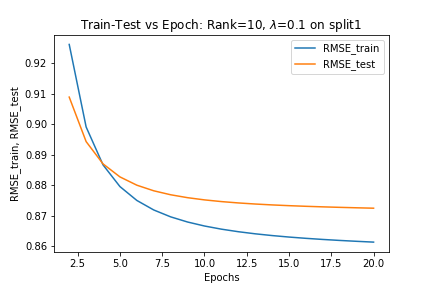
\includegraphics[width=4cm, height=4cm]{plots/train_test_vs_epoch_split1_rank_10_lambd_0_1.png}
%	\includegraphics[width=4cm, height=4cm]{plots/split_1_RMSE_epoch__rank_10_lambd_0_02.png}
%	\includegraphics[width=4cm, height=4cm]{plots/split_1_RMSE_epoch__rank_10_lambd_1_0.png}
%	\includegraphics[width=4cm, height=4cm]{plots/split_1_RMSE_epoch__rank_10_lambd_0_1.png}
	\caption{Example of an image with acceptable resolution}
	\label{fig:hires-photo}
\end{figure}

\subsection{Figure Captions}

Figures must be numbered using Arabic numerals.  Figure captions must
be in 8 pt Regular font.  Captions of a single line (e.g. Fig.
\ref{fig:lores-photo}) must be centered whereas multi-line captions
must be justified (e.g. Fig.  \ref{fig:sample_graph}).  Captions with
figure numbers must be placed after their associated figures, as shown
in Fig. \ref{fig:sample_graph}.

\subsection{Table Captions}

Tables must be numbered using uppercase Roman numerals.  Table
captions must be centred and in 8 pt Regular font with Small Caps.
Every word in a table caption must be capitalized except for short
minor words as listed in Section \ref{sec:title and author details}.
Captions with table numbers must be placed before their associated
tables, as shown in Table \ref{tab:font-sizes}.

\subsection{Page Numbers, Headers and Footers}

Page numbers, headers and footers must not be used.

\subsection{Links and Bookmarks}

All hypertext links and section bookmarks will be removed from
papers during the processing of papers for publication.  If you
need to refer to an Internet email address or URL in your paper,
you must type out the address or URL fully in Regular font.

\subsection{References}

The heading of the References section must not be numbered.
All reference items must be in 8 pt font.  Please
use Regular and Italic styles to distinguish different fields as
shown in the References section. Number the reference items
consecutively in square brackets (e.g. \cite{IEEEexample:book}).

When referring to a reference item, please simply use the
reference number, as in \cite{IEEEexample:bookwithseriesvolume}.
Do not use �Ref. \cite{IEEEexample:article_typical}� or
�Reference \cite{IEEEexample:article_typical}� except at the
beginning of a sentence, e.g.  ``Reference
\cite{IEEEexample:article_typical} shows �''.  Multiple
references are each numbered with separate brackets (e.g.
\cite{IEEEexample:bookwithseriesvolume},
\cite{IEEEexample:article_typical},
\cite{IEEEexample:confwithpaper}--[6]).

Examples of reference items of different categories shown in the
References section include:

\begin{itemize}
\item	example of a book in \cite{IEEEexample:book}
\item	example of a book in a series in \cite{IEEEexample:bookwithseriesvolume}
\item	example of a journal article in \cite{IEEEexample:article_typical}
\item	example of a conference paper in \cite{IEEEexample:confwithpaper}
\item	example of a patent in \cite{IEEEexample:uspat}
\item	example of a website in \cite{IEEEexample:IEEEwebsite}
\item	example of a web page in \cite{IEEEexample:shellCTANpage}
\item	example of a databook as a manual in \cite{IEEEexample:motmanual}
\item	example of a datasheet in \cite{IEEEexample:datasheet}
\item	example of a master's thesis in \cite{IEEEexample:masterstype}
\item	example of a technical report in \cite{IEEEexample:techreptype}
\item	example of a standard in \cite{IEEEexample:standard}
\end{itemize}

% the following command shrinks the final page to force the columns to
% be balanced.  You will need to adjust the value according to the 
% appearance of your last page.  Start by setting the value to 0mm
% and slowly increase it until the columns balance.  Alternatively,
% use balance.sty to do the job.
\enlargethispage{-62mm}

\section{Conclusion}

The version of this template is V3.  Most of the formatting
instructions in this document have been compiled by Causal Productions
from the IEEE LaTeX style files.  Causal Productions offers both A4
templates and US Letter templates for LaTeX and Microsoft Word.  The
LaTeX templates depend on the official IEEEtran.cls and IEEEtran.bst
files, whereas the Microsoft Word templates are self-contained.
Causal Productions has used its best efforts to ensure that the
templates have the same appearance.

Causal Productions permits the distribution and revision of these
templates on the condition that Causal Productions is credited in the
revised template as follows: ``original version of this template was
provided by courtesy of Causal Productions
(www.causalproductions.com)''.

\section*{Acknowledgment}

The heading of the Acknowledgment section and the References section
must not be numbered.

Causal Productions wishes to acknowledge Michael Shell and other
contributors for developing and maintaining the IEEE LaTeX style files
which have been used in the preparation of this template.  To see the
list of contributors, please refer to the top of file IEEETran.cls in
the IEEE LaTeX distribution.

\bibliographystyle{IEEEtran}

\bibliography{IEEEabrv,IEEEexample}

\end{document}
